
\section{Introduction}

\iffalse
Outline: 
1. LLM reasoning capacity => external tools => agents; Deep research agent is important and popular
2. High performance comes at time efficiency: (1) extensive token costs for reasoning (2) sequential nature of 
mutli-turn reasoning-action-observation. Should we have a profiling of reasoning time and functional call time?
    - It typically requires a strong model with high parameter capacity and long reasoning 
3. latency is very critical for users, especially deep research agents. 
4. Corroborating with recent works, we find that action is the right barrier for speculation and verification 
5. However, how to speculative and how to verify to balance the accuracy and efficiency is challenging 
   - How to improve the accuracy of speculation => thus the verification pass rate higher => higher efficiency
   - How to verify smartly, to ensure the agent performance is not compromised 
6. Our observation: different actions require different speculation strategies for the agent to be efficient and accurate
   - Search action: high uncertainty, underspecified query => need strong reasoning to reduce the uncertainty => smaller model with reasoning 
   - Visit action: low uncertainty, concrete content => strong parametric prior is more important => large model without reasoning 
   - This is aligned with system 1 and system 2 thinking in cognitive science 
   - We prove this with entropy analysis of different actions and end-to-end experiments
7. Our framework: Heterogeneous speculation framework for deep research agents 
   - Draft model: smaller model with reasoning for system 2 action; large model without reasoning for system 1 action
   - verification model: large model judge
8. Evaluation results
8. Contributions

Outline
1. In this work, we rethink the speculate-verify paradigm for deep research agents by carefully analyzing action heterogeneity and verification trade-offs.

2. Our goal is to improve the accuracy of action speculation to improve the acceptance ratio and thus enhance the efficiency, while designing effective verification to maintain the agent performance.

3. We observe that, to predict next action more accurately, different actions require different speculation strategies based on their distinct characteristics and demands.
    - Deep research agents mainly involve two types of actions: Search and Visit, where a search action issue a query to the search engine to retrieve relevant webpages (URL lists), while a visit action access a specific webpage to extract its content.
    - We find that generating a high-quality Search action demands strong reasoning capabilities to reduce the inherent uncertainty in query formulation, while Visit actions benefit more from robust parametric knowledge and less from explicit reasoning because it only requires choose one specific URL from a concrete list, with less action space. 
    - We confirms this with an entropy-based analysis of action decisions and end-to-end studies.
    - This is similar to the cognitive science distinction between \textit{System 2} (deliberative) and \textit{System 1} (intuitive) decision making, where search aligns with System 2 behavior and visit with System 1 behavior.
    - There are typically two lightweight speculation methods: small model with reasoning and large model which directly generates actions without reasoning.
    - According to the above property, using a small model with reasoning to draft search action and a large model without reasoning to draft visit action can yield higher speculation accuracy.

4. The verification design should be also carefully considered to ensure high efficiency and the agent performance is not compromised. Do the exact action match is too strict because two queries generated by different models can be semantically similar but not exactly the same. Moreover, do the action match requires the base model to first finish its reasoning, which can be time-consuming and delay the verification process. 

Given the above observations and challenges, we propose \method, a heterogeneous action speculation framework for deep research agents.

- Our method: the critical path does not have base model reasoning
\fi

% The increasing reasoning capabilities of Large Language Models (LLMs) enables them to interact with external tools and environments, facilitating the development of intelligent agents~\cite{yao2022react,shinn2023reflexion}.
% Notably, deep research agents have emerged as a prominent application to solve open-ended, long-horizon research tasks with high information-seeking and reasoning demands~\cite{deepresearch}.  
% Through the multi-step reasoning and tool-use paradigm, these agents continuously gather evidence from external resources such as search engines and refine hypotheses iteratively, moving beyond static question answering to tackling complex research problems. 

The increasing reasoning capabilities of large language models (LLMs) enable interaction with external tools and environments, driving the development of intelligent agents~\cite{yao2022react,shinn2023reflexion,schick2023toolformer}.
Among these, deep research agents have emerged as a prominent application for addressing open-ended, long-horizon research tasks with high information-seeking and reasoning demands~\cite{deepresearch}.
By iteratively reasoning and invoking external tools such as search engines, these agents accumulate evidence and refine hypotheses, extending beyond static question answering to complex research problems.

\begin{figure}
    \centering
    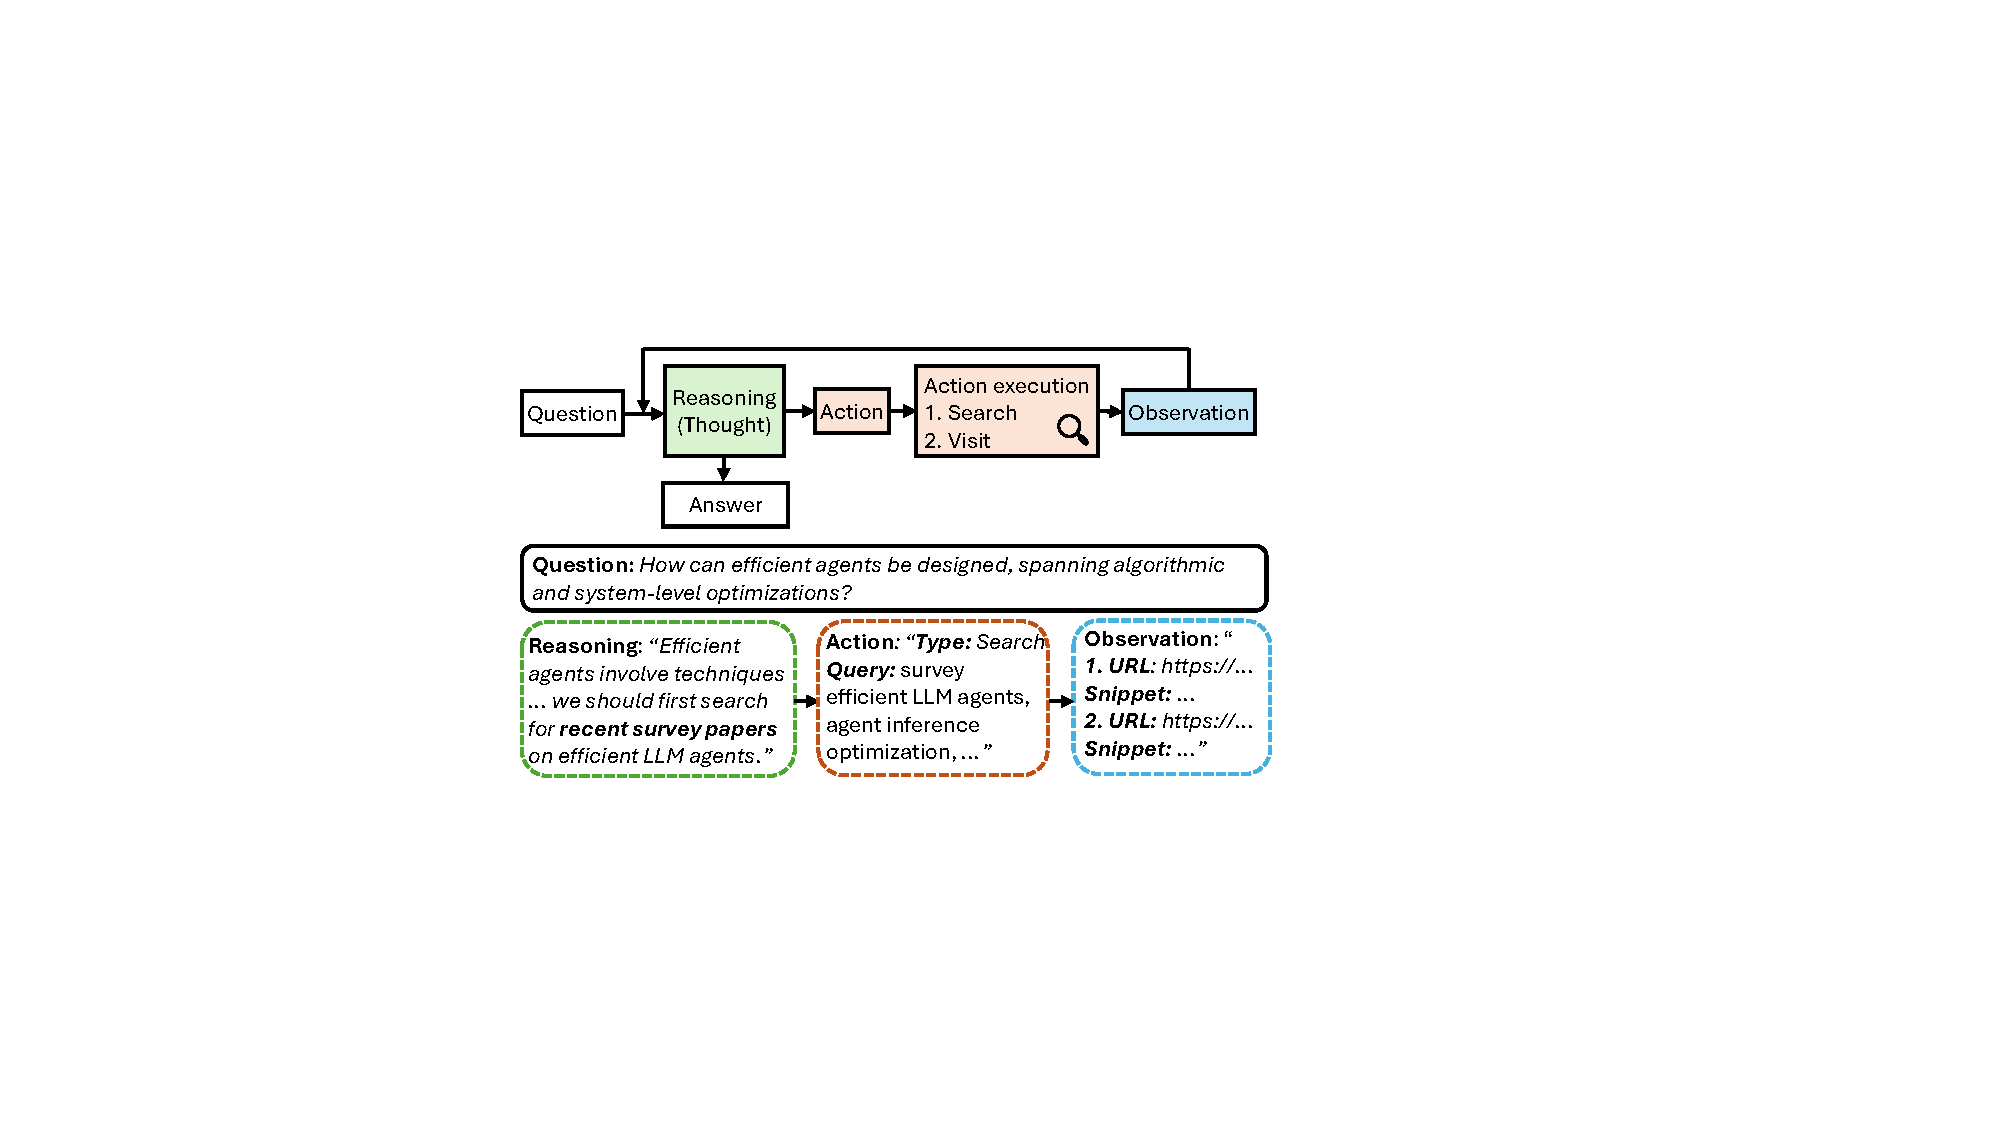
\includegraphics[width=\linewidth]{figs/deep_research.pdf}
    \caption{Deep research agent workflow. Deep research agents follow a Reason-Action-Observation loop, where the agent alternates between generating reasoning traces and executing actions (Search or Visit) to gather information.}
    \label{fig:deep_research}
\end{figure}


% Despite its advancements, deep research agents often suffer from high inference latency.
% As shown in Figure~\ref{fig:deep_research}, LLM agent often follows the Reason-Action (ReAct) paradigm \cite{yao2022react} with 
% a strict sequential dependency: the model must synthesize a complete reasoning trace 
% before emitting an executable action and then, wait for the subsequent observations before moving forward to the next reasoning phase. 
% Both the reasoning process and the action execution can be time-consuming, especially when the agent relies on large models with extensive token usage for reasoning and interacts with external tools that may have variable response times.
% The reasoning-action-observation cycle repeats for multiple turns until the agent reaches a final answer, 
% often requiring minutes, if not hours, to answer a single query. 

Despite their effectiveness, deep research agents often incur high inference latency.
As shown in Figure~\ref{fig:deep_research}, agents typically follow the ReAct paradigm~\cite{yao2022react} with strict sequential dependencies: the model must complete a reasoning trace before emitting an action and then wait for the resulting observation before proceeding.
Both reasoning and action execution can be time-consuming, particularly when using large models with long reasoning traces and external tools with variable response times\cite{kim2023llm,zhang2025optimizing}.
This reasoning--action--observation cycle repeats over many turns until a final answer is produced, often requiring minutes or longer for a single query.


% To mitigate this inefficiency, a promising direction is to leverage the speculate-verify paradigm, in which a lightweight model or strategy speculates the next action and executes it immediately, while the base model concurrently performs its reasoning process~\cite{huang2025reducing,guan2025dynamic}.
% If the base model generates an action consistent with the speculative one, 
% it skips the action execution and directly accept the speculative tool call response (observation), saving the latency; when they disagree, the base model executes as usual.
% This paradigm differs from, and complements, speculative decoding~\cite{leviathan2023fast}, as it operates at the level of agent actions rather than language tokens, enabling latency reduction through parallelism between reasoning and tool use.
% However, a fundamental challenge lies in how to design effective speculation and verification strategies that balance the agent efficiency and accuracy.
% Inaccurate next-action prediction or conservative verification can lead to frequent fallbacks to the base model, diminishing efficiency gains, while overly permissive verification risks degrading the agent's overall performance.

A promising approach to reduce latency is the speculate--verify paradigm, where a lightweight model or strategy speculates the next action and executes it immediately, while the base model concurrently performs its reasoning~\cite{huang2025reducing,guan2025dynamic}.
If the base model's action matches the speculative one, the speculative observation is directly accepted, saving execution time; otherwise, the base model executes the action as usual.
Unlike speculative decoding~\cite{leviathan2023fast}, this approach operates at the action level rather than the token level, enabling parallelism between reasoning and tool use.
However, designing effective speculation and verification remains challenging: inaccurate speculation or conservative verification leads to frequent fallbacks and limited speedups, whereas overly permissive verification risks degrading agent performance.


% In this work, we rethink the speculate--verify paradigm for deep research agents through a principled analysis of action heterogeneity and verification trade-offs.
% The lightweight speculation approaches typically fall into two categories: (i) small models with explicit reasoning, and (ii) large models that directly emit actions without reasoning.
% We observe that different action types exhibit markedly different uncertainty profiles and thus call for distinct speculation strategies.
% In particular, deep research agents predominantly rely on two actions: Search and Visit.
% A Search action formulates a query to retrieve a list of relevant webpages, whereas a Visit action selects and accesses a specific URL from the candidate set.
% We find that generating effective Search actions requires strong reasoning to resolve high uncertainty in query formulation, while Visit actions operate over a much more constrained action space and rely primarily on parametric knowledge, with limited need for explicit reasoning.


In this work, we rethink speculate--verify for deep research agents through a principled analysis of action heterogeneity and verification trade-offs.
Existing lightweight speculation methods generally adopt either (i) small models with explicit reasoning or (ii) large models that emit actions without reasoning.
We observe that different action types exhibit distinct uncertainty profiles and thus require different speculation strategies.
Deep research agents primarily use two actions: \textit{Search}, which formulates a query to retrieve relevant webpages, and \textit{Visit}, which selects and accesses a specific URL from a candidate set.
Search involves high uncertainty in query formulation and benefits from strong reasoning, whereas Visit operates over a constrained action space and relies mainly on parametric knowledge.


% We substantiate this distinction through an entropy-based analysis of action decision-making with and without reasoning, complemented by end-to-end empirical studies.
% Our results consistently show that Search actions exhibit higher uncertainty than Visit actions, and explicit reasoning helps reduce uncertainty for Search but yields marginal benefits for Visit.
% This finding closely mirrors the cognitive science dichotomy between \textit{System~2} (deliberative) and \textit{System~1} (intuitive) thinking mode, with Search aligning with the former and Visit with the latter.
% Motivated by these insights, we show that aligning speculation mechanisms with action characteristics -- using a small reasoning model for Search and a large model without explicit reasoning for Visit -- significantly improves speculation accuracy.

We validate this distinction via end-to-end empirical evaluations, together with an entropy-based analysis of action decisions with and without reasoning.
Across settings, Search actions exhibit much higher uncertainty than Visit actions; explicit reasoning helps reduce uncertainty for Search but provides marginal gains for Visit.
This pattern aligns with the cognitive science distinction between \textit{System~2} (deliberative) and \textit{System~1} (intuitive) reasoning, with Search corresponding to the former and Visit to the latter.
Guided by these insights, we show that matching speculation strategies to action characteristics -- using a small reasoning model for Search and a large model without reasoning for Visit -- significantly improves speculation accuracy.

% Beyond speculation, verification also plays an critical role in achieving high efficiency without sacrificing agent performance.
% Exact action matching is often overly restrictive: two actions may be semantically equivalent despite token-level differences, especially for Search queries.
% Moreover, action-based verification -- whether exact or approximate -- typically requires the base model to complete its full reasoning process before verification can occur, placing reasoning on the critical path and limiting potential latency reductions.

Verification is also critical for achieving efficiency without sacrificing performance.
Exact action matching is often overly restrictive, as semantically equivalent actions, especially queries, may differ at the token level.
Moreover, action-based verification typically requires the base model to complete reasoning before verification, placing reasoning on the critical path and limiting latency reductions.


% Based on these observations, we propose \method, a heterogeneous action speculation framework for deep research agents that tailors speculation and verification to action-specific properties.
% \method~employs a small reasoning model to speculate actions, while allowing the large base model to concurrently generate a Visit action without explicit reasoning.
% If the speculative action is Search, the agent adopts the small model's output as the draft; otherwise, it uses the base model's directly generated Visit action.
% For verification, rather than performing explicit action matching, \method~leverages the base model's internal confidence to determine whether to accept the drafted action, thereby removing the base model's reasoning from the critical path.

Based on these observations, we propose \method, a heterogeneous action speculation framework for deep research agents that tailors speculation and verification to action-specific properties.
\method~uses a small reasoning model to speculate actions, while allowing the base model to concurrently generate a Visit action by skipping reasoning.
It dynamically selects an appropriate draft based on the reasoning state.
For verification, \method~leverages the base model's internal confidence rather than explicit action matching, removing base-model reasoning from the critical path while preserving the agent performance.

% We implement \method~and evaluate its accuracy and efficiency on two representative reasoning models, MiroThinker~\cite{team2025mirothinker} and Qwen-3~\cite{team2025tongyi}, using widely used deep research benchmarks, including GAIA-Text-103~\cite{wu2025webdancer}, XBench\_DeepSearch~\cite{chen2025xbench} and Seal-0~\cite{pham2025sealqa}.
% Our results show that \method~achieves up to \textbf{3.28}$\times$ end-to-end latency speedup while maintaining performance comparable to the base model with full reasoning.

We implement \method~and evaluate it on two representative reasoning models, MiroThinker~\cite{team2025mirothinker} and Qwen-3~\cite{team2025tongyi}, using popular deep research benchmarks including GAIA-Text-103~\cite{wu2025webdancer}, XBench-DeepSearch~\cite{chen2025xbench}, and Seal-0~\cite{pham2025sealqa}.
\method~achieves up to \textbf{3.28}$\times$ end-to-end latency speedup while maintaining performance comparable to the fully reasoning base model.





\iffalse
Initial draft:

Recent advances in Large Language Models (LLMs) have given rise to deep research agents. These agents can perform multi-step reasoning and seeking information across the internet, allowing them to gather evidence and iteratively refine intermediate hypotheses\cite{team2025mirothinker,team2025tongyi}.
This iterative process of reasoning and interaction allows agents to move beyond static question answering and address increasingly complex, long-horizon research tasks.

However, the advancements of deep research agents often incur a substantial latency overhead. This bottleneck can be derived from the Reason–Action (ReAct) paradigm\cite{yao2022react}, which enforces a strict sequential dependency: the model must synthesize a complete reasoning trace before emitting an executable action and awaiting the subsequent observation. As a result, the agent cannot begin interacting with the environment until it has fully completed its internal reasoning for the current step.

To mitigate this inefficiency, recent works have proposed a range of latency-oriented optimizations. 
A common strategy is to leverage lightweight inference methods for most steps, while selectively invoking original reasoning only when needed\cite{guan2025dynamic}. Such lightweight approaches include delegating inference to smaller or quantized models\cite{bian2025limits}, or skipping the reasoning process entirely\cite{huang2025reducing}.

Despite their effectiveness, existing approaches largely adopt a homogeneous view of agent actions and apply a uniform lightweight strategy across all actions. They use a same lightweight method for all of the actions. Such designs often yield inaccurate or underpowered decisions, proving ineffective in practice by either triggering frequent fallback to high-capacity models or resulting in longer exploration trajectories \cite{lin2025towards}.

In this work, we make a simple yet underexplored observation: deep research agents involve two types of actions, Search and Visit. A Search action issues queries to search engines (e.g., Google or Bing) to retrieve relevant webpages. A Visit action accesses webpages or local files and extracts or summarizes their content. Search actions require the agent to translate underspecified goals into effective queries. This process typically demands explicit reasoning and exhibits high uncertainty.
In contrast, Visit actions operate on concrete retrieved content, involving localized decisions such as selecting, filtering, or extracting relevant information, which tend to be more deterministic and rely primarily on parametric knowledge.

This asymmetry mirrors a well-established distinction between deliberative and intuitive decision making.
From the perspective of \textit{System 2} versus \textit{System 1}, Search aligns with \textbf{System 2} behavior, emphasizing \textbf{reasoning depth} over model scale, whereas Visit corresponds to \textbf{System 1} behavior, relying primarily on \textbf{parametric capacity} rather than explicit logical reasoning.
 
Motivated by this observation, we propose \method, a collaboration framework that generates System 1 and System 2 actions heterogeneously based on their different inference demands. Rather than uniformly using the same lightweight method, \method dynamically assigns deliberative reasoning with smaller model to cognitively demanding System 2 actions, while executing System 1 actions using the origin full-size model but without the reasoning process.
Our contributions can be summarized as follows:

\begin{itemize}
    \item We identify a fundamental action-level asymmetry in deep research agents by analyzing the entropy of action decisions. We show that \textit{System 2} actions (e.g., Search) exhibit high initial uncertainty, where explicit reasoning plays a critical role in reducing action entropy, whereas \textit{System 1} actions (e.g., Visit) naturally operate in low-entropy regimes and gain little from reasoning, instead benefiting from strong parametric priors.
    
    \item We propose \method, a heterogeneous collaboration framework that decouples \textit{System 2} and \textit{System 1} actions in agent execution. \method assigns a smaller model with explicit reasoning to handle \textit{System 2} actions, while using the original full-size model to directly generate \textit{System 1} actions without reasoning, and selectively escalates to full reasoning with the large model when necessary.
    
    \item We implement the \method  on top of MiroThinker and SGLang and demonstrate up to $xxx\times$ speedup over prior-art collaboration frameworks without compromising accuracy.
\end{itemize}
\fi